\documentclass[mathNotesPreamble]{subfiles}
\begin{document}
\relscale{1.4} %TODO
\section{16.5: Triple Integrals in Cylindrical and Spherical Coordinates}

  \begin{thmBox*}[Transformations between Cylindrical and Rectangular Coordinates]
    \vspace*{0.5\baselineskip}
    \begin{minipage}{0.5\linewidth}
      \begin{center}
        \textbf{Rectangular} $\rightarrow$ \textbf{Cylindrical}
      \end{center}
      \begin{align*}
        r^2&=x^2+y^2\\
        \tan\theta&=y/x\\
        z&=z
      \end{align*}
    \end{minipage}%
    \begin{minipage}{0.5\linewidth}
      \begin{center}
        \textbf{Cylindrical} $\rightarrow$ \textbf{Rectangular}
      \end{center}
      \begin{align*}
        x&=r\cos\theta\\
        y&=r\sin\theta\\
        z&=z
      \end{align*}
    \end{minipage}%
  \end{thmBox*}

  \begin{thmBox*}[Theorem 16.6: Change of Variables for Triple Integrals in Cylindrical Coordinates]
    Let $f$ be continuous over the region $D$, expressed in cylindrical coordinates as
      \[D=\set{(r,\theta,z): 0\leq g(\theta)\leq r\leq h(\theta),\ \alpha\leq \theta\leq \beta,\ G(x,y)\leq z\leq H(x,y)}\]
    Then $f$ is integrable over $D$, and the triple integral of $f$ over $D$ is
      \[\iiint\limits_D f(x,y,z)\,dV=\int_\alpha^\beta \int_{g(\theta)}^{h(\theta)}\int_{G\parens{r\cos\theta),\ r\sin(\theta)}}^{H\parens{r\cos\theta),\ r\sin(\theta)}}f\parens{r\cos\parens{\theta}, r\sin\parens{\theta}}\,dz\,r\,dr\,d\theta.\]
  \end{thmBox*}

  \begin{thmBox*}[Transformations between Spherical and Rectangular Coordinates]
    \vspace*{0.5\baselineskip}
    \begin{minipage}{0.5\linewidth}
      \begin{center}
        \textbf{Rectangular} $\rightarrow$ \textbf{Spherical}
      \end{center}
      \begin{align*}
        \rho^2&=x^2+y^2+z^2\\
        &\hspace*{-15pt}\textnormal{Use trigonometry to find}\\
        &\hspace*{-15pt}\varphi \textnormal{ and } \theta.
      \end{align*}
    \end{minipage}%
    \begin{minipage}{0.5\linewidth}
      \begin{center}
        \textbf{Spherical} $\rightarrow$ \textbf{Rectangular}
      \end{center}
      \begin{align*}
        x&=\rho\sin(\varphi)\cos(\theta)\\
        y&=\rho\sin(\varphi)\sin(\theta)\\
        z&=\rho\cos(\varphi)
      \end{align*}
    \end{minipage}%
  \end{thmBox*}

  \pagebreak
  \begin{center}
  %https://tex.stackexchange.com/questions/337570/tabularx-with-different-column-widths
    \renewcommand{\tabularxcolumn}[1]{m{#1}} %sets columns to vertically centered
    \relscale{0.775}
    \begin{tabularx}{\linewidth}{@{}
      >{\hsize=0.575\hsize}X@{\hspace*{20pt}}
      >{\hsize=1.80\hsize}X@{\hspace*{20pt}}
      >{\hsize=0.625\hsize}Y}\toprule
      \textbf{Name}& 
      \textbf{Description}& 
      \textbf{Example}\\\midrule
      %
      Sphere, radius $a$, center $(0,0,0)$&
      $\set{(\rho, \varphi, \theta): \rho=a}, a>0$&
      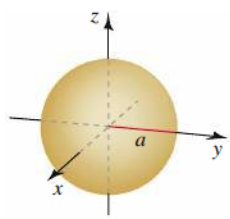
\includegraphics[width=0.525\linewidth]{images/briggs_16_05/table16p5_sphere}\\
      %
      Cone&
      $\set{(\rho,\varphi, \theta): \varphi=\varphi_0}, \varphi_0\neq 0, \pi/2, \pi$&
      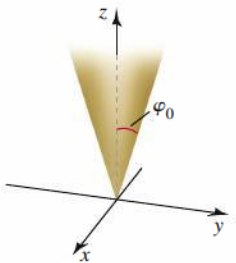
\includegraphics[width=0.525\linewidth]{images/briggs_16_05/table16p5_cone}\\
      %
      Vertical\newline half-plane&
      $\set{(\rho,\varphi, \theta): \theta=\theta_0}$&
      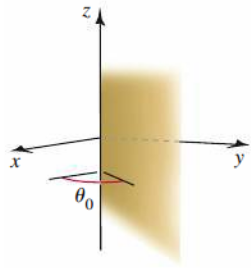
\includegraphics[width=0.525\linewidth]{images/briggs_16_05/table16p5_vertHalfPlane}\\
      %
      Horizontal\newline plane, $z=a$&
      $a>0: \set{(\rho,\varphi, \theta): \rho=a\sec(\varphi),\ 0\leq \varphi< \pi/2}$\newline
      $a<0: \set{(\rho,\varphi, \theta): \rho=a\sec(\varphi),\ \pi/2< \varphi\leq \pi}$&
      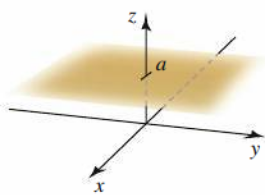
\includegraphics[width=0.525\linewidth]{images/briggs_16_05/table16p5_horizHalfPlane}\\
      %
      Cylinder,\newline radius $a>0$&
      $\set{(\rho,\varphi, \theta): \rho=\alpha\csc(\varphi),\ 0<\varphi<\pi}$&
      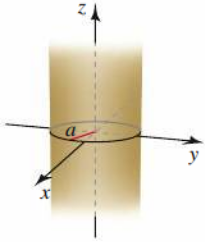
\includegraphics[width=0.525\linewidth]{images/briggs_16_05/table16p5_cylinder}\\
      %
      Sphere,\newline radius $a>0$\newline center $(0,0,a)$&
      $\set{(\rho,\varphi, \theta): \rho=2a\cos(\varphi),\ 0\leq\varphi\leq\pi/2}$&
      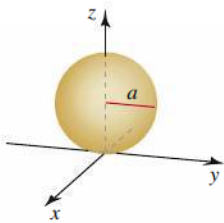
\includegraphics[width=0.525\linewidth]{images/briggs_16_05/table16p5_sphereOffset}\\
      \bottomrule
    \end{tabularx}
  \end{center}
  \pagebreak

  \begin{thmBox*}[Theorem 16.7: Change of Variables for Triple Integrals in Spherical Coordinates]
    Let $f$ be continuous over the region $D$, expressed in spherical coordinates as
      \[D=\set{(\rho,\varphi,\theta): 0\leq g(\varphi,\theta)\leq \rho\leq h(\varphi,\theta),\ a\leq \varphi\leq b,\ \alpha\leq \theta\leq \beta}.\]
    Then $f$ is integrable over $D$, and the triple integral of $f$ over $D$ is
    \begin{align*}
      \mathrlap{\iiint\limits_D f(x,y,z)\,dV}&\\
      &=\int_\alpha^\beta \int_a^b \int_{g(\varphi,\theta)}^{h(\varphi,\theta)}f\parens{\rho\sin(\varphi)\cos(\theta),\,\rho\sin(\varphi)\sin(\theta),\,\rho\cos(\varphi)}\rho^2 \sin(\varphi)\ d\rho\,d\varphi\,d\theta.
    \end{align*}
  \end{thmBox*}

  \pagebreak
  
\end{document}